\documentclass[12p,a4paper]{article}
\usepackage[utf8]{inputenc}
\usepackage[T1]{fontenc,url}
\usepackage{parskip}
\usepackage{lmodern}
\usepackage{microtype}
\usepackage{verbatim}
\usepackage{amsmath, amssymb}
\usepackage{tikz}
\usepackage{physics}
\usepackage{mathtools}
\usepackage{algorithm}
\usepackage{algpseudocode}
\usepackage{listings}
\usepackage{enumerate}
\usepackage{graphicx}
\usepackage{float}
\usepackage{epigraph}
\usepackage{hyperref}
\usepackage{tikz}
\usepackage[a4paper]{geometry}
\begin{document}


\newcommand{\half}{\frac{1}{2}}
\renewcommand{\exp}[1]{\mathrm{e}^{#1}}
\renewcommand{\i}{\mathrm{i}}
\newcommand{\R}{\mathbb{R}}

\newgeometry{left = 0cm, bottom = 0cm, top = 0cm, right = 0cm}

\begin{tikzpicture}[]
\node at (0,0) {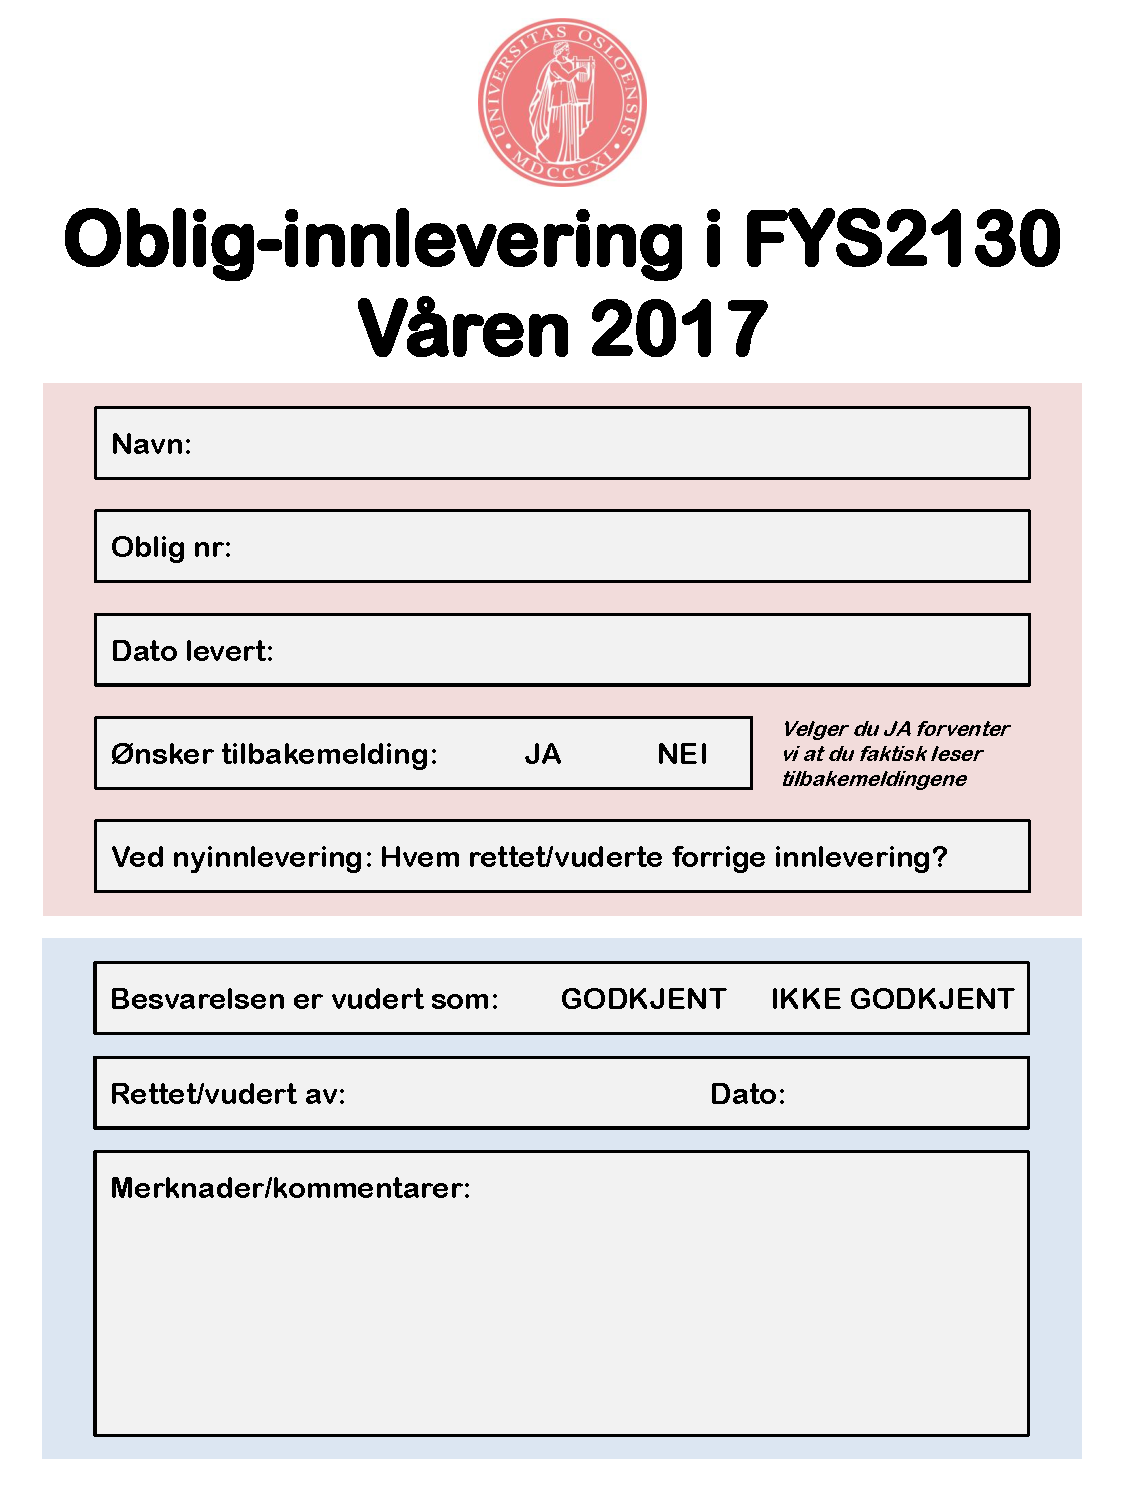
\includegraphics[width=\textwidth]{../oblig_forside_2017.pdf}};
\node[right] at (-7,5.7) {\begin{huge} Jonas Gahr Sturtzel Lunde \end{huge}};
\node[right] at (-6.3,3.77) {\begin{huge} 4 \end{huge}};
\node[right] at (-5.4,1.85) {\begin{huge} 21.02.2017 \end{huge}};
\draw(-0.35,-0.05) circle[radius = 0.5cm];
\end{tikzpicture}

\pagebreak
\restoregeometry 


\section*{Oppgave 2}\label{sec:2}
Når vi kommer over halvparten av samplingsfrekvensen, altså i dette tilfellet rundt $22$kHz, har vi ikke lenger høy nok oppløsning til at de harmoniske svingningene blir tolket på en entydig måte. Hvis vi ikke representerer bølgene med høy nok oppløsning vil de kunne fremstå som bølger med lavere frekvens, fordi vi rett og slett "hopper over" en eller flere bølgetopper mellom hvert punkt i vår digitale fremstilling.

I dette tilfellet vil det bety at lyder over $22$kHz kan komme til å avspilles som en helt tilfeldig lavere frekvens, og fremstå som tilfeldig støy.


\section*{Oppgave 8}
Vi bruker den diskretiserte definisjonen av fourier-transformasjon til å se på den første frekvensen, $k=0$, eller 0Hz, i frekvensspekteret.
\begin{align*}
X_k &= \frac{1}{N} \sum\limits_{n=0}^{N-1} x_n \exp{-i\frac{2\pi}{N}kn} \\
X_0 &= \frac{1}{N} \sum\limits_{n=0}^{N-1} x_n \exp{-i\frac{2\pi}{N}0n} = \frac{1}{N} \sum\limits_{n=0}^{N-1} x_n \\
&= \frac{x_0 + x_1 + \cdots + x_{n-2} + x_{n-1}}{N}
\end{align*}
Vi ser at dette er gjennomsnittet av de $N$ verdiene til $x_n$.\footnote{Interessant bemerkning: Dette utarter seg i den originale funksjonen som et konstantledd, ettersom at sinus og cosinus av en frekvens på 0Hz er en konstant. Dette betyr at informasjon om hvor forskjøvet de harmoniske svingningen er fra $x=0$ ligger i $X_0$. Ettersom dette er harmoniske svingninger, vil selvsagt en slik forskyvning tilsvare gjennomsnittsverdien av funksjonen, som er 0 når svingningen ikke har et konstantledd.}

\pagebreak

Som vi ser fra figur \ref{fig:average} stemmer dette. $X_k$ for $k=0$ er gjennomsnittet av $x_n$.

\begin{figure}[H]
\centering
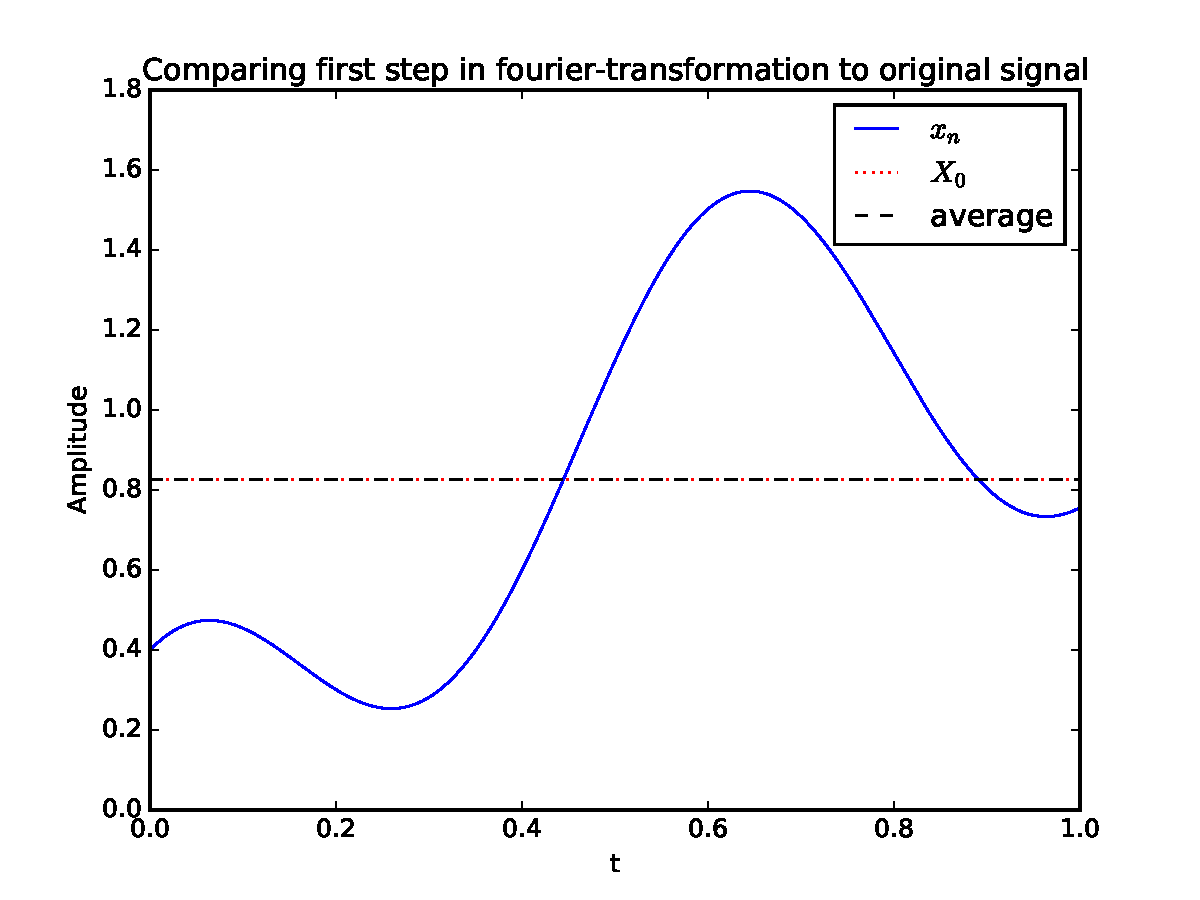
\includegraphics[width=0.8\textwidth]{fig/average.pdf}
\caption{Første steg i diskret Fourier-transformasjon}
\label{fig:average}
\end{figure}


\section*{Oppgave 9}

Som vi ser fra figur \ref{fig:100Hz} til \ref{fig:400Hz} at frekvensbildet stemmer overens med frekvensen vi satt i cosinusfunksjonen. Fra figur \ref{fig:700Hz} til \ref{fig:1300Hz} ser vi derimot at frekvensbildet er feil. Dette er fordi fouriertransformasjonen bare kan benyttes på harmoniske svingninger med frekvens under halvparten av samplingfrekvensen, som poengtert i oppgave 2. Denne har vi satt til $1000Hz$, og frekvenser over $500Hz$ vil derfor opptre med for lav oppløsning til å kunne representeres nøyaktig, som skaper et misvisende frekvensbilde.

Jeg vet ikke om dette var poenget med oppgaven, men jeg skjønner ærlig talt ikke hva "et system i hvor linjene kommer ut i frekvensspekteret" skal bety. Jeg plotter et frekvensspekter, selvsagt kommer linjene ut i frekvensspekteret. Hvor ellers skulle de kommet ut? 

\begin{figure}[H]
\centering
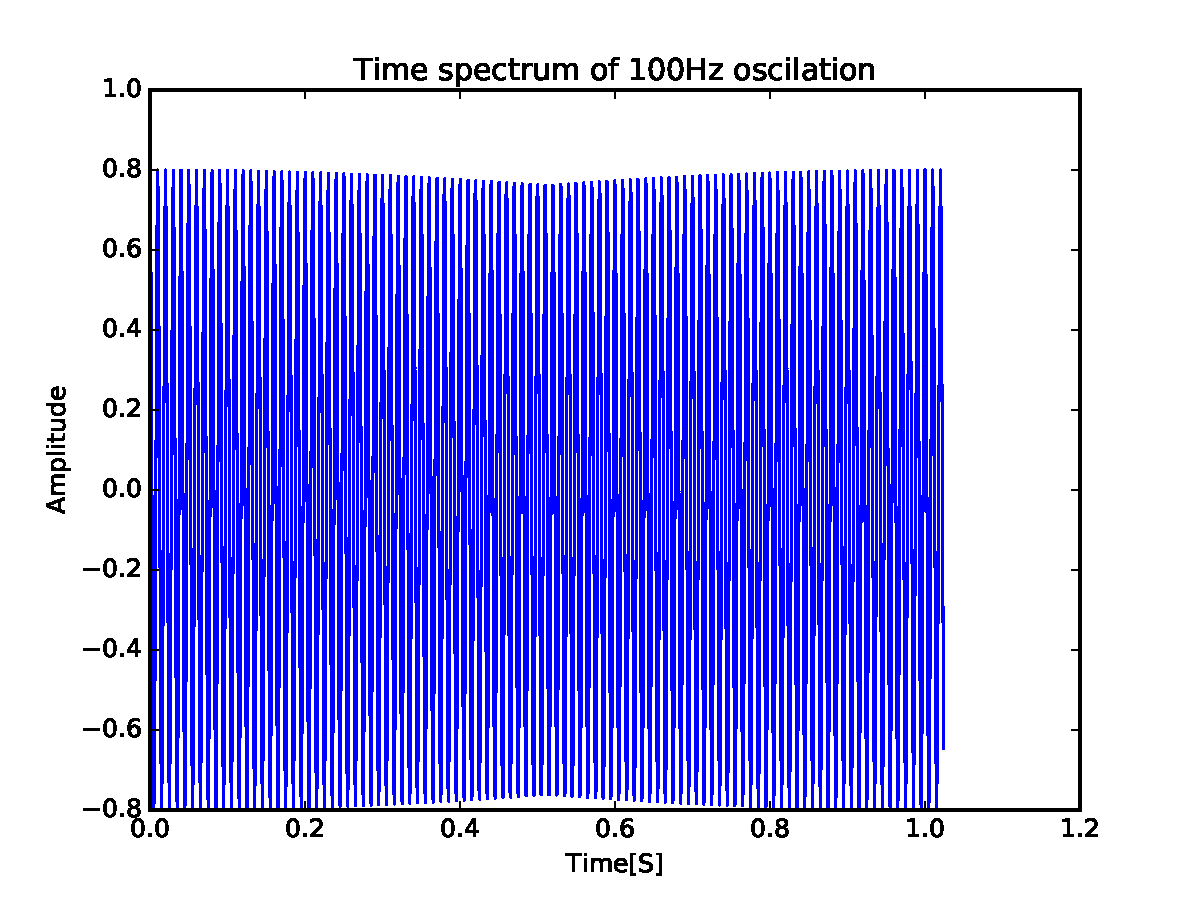
\includegraphics[width=0.49\textwidth]{fig/timespec100.pdf}
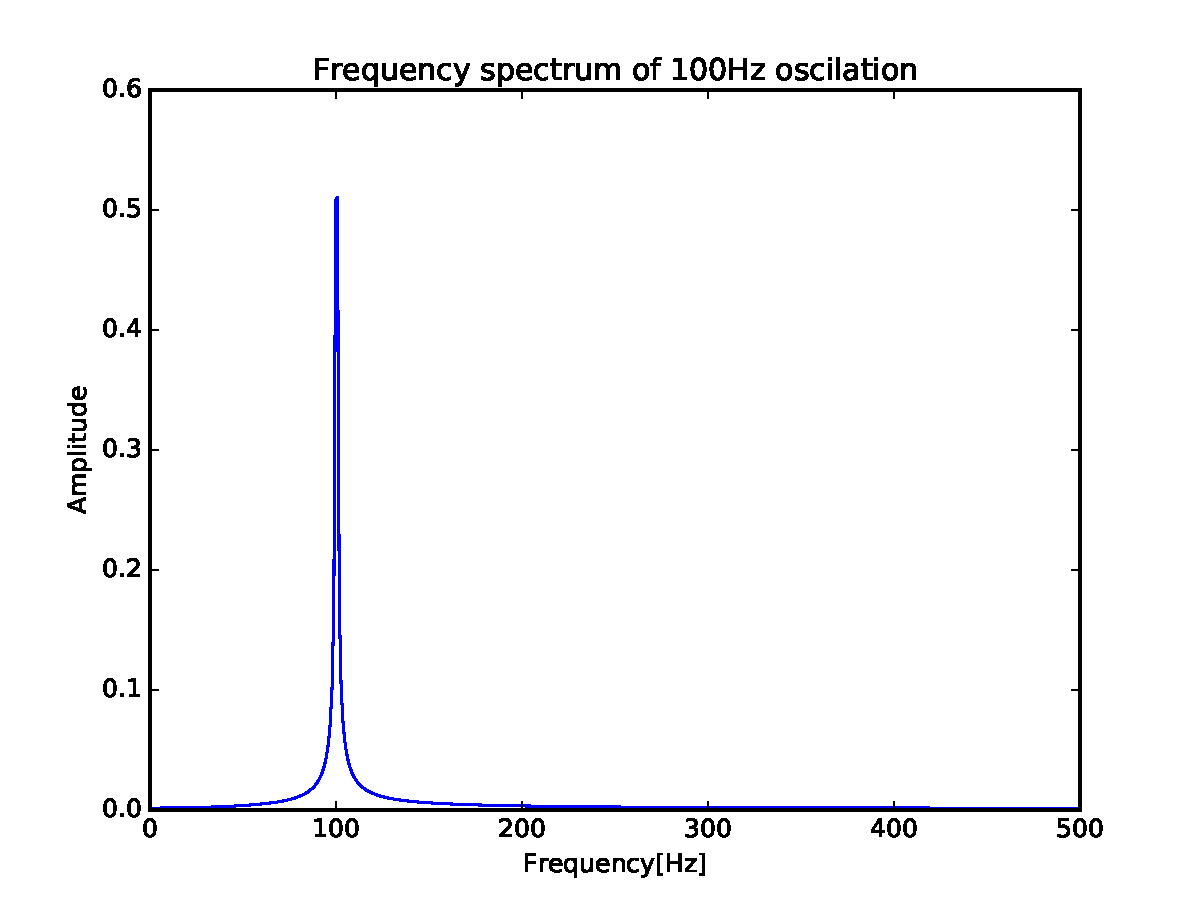
\includegraphics[width=0.49\textwidth]{fig/freqspec100.pdf}
\caption{Tids- og frekvensspekter av 100Hz svingning}
\label{fig:100Hz}
\end{figure}
\begin{figure}[H]
\centering
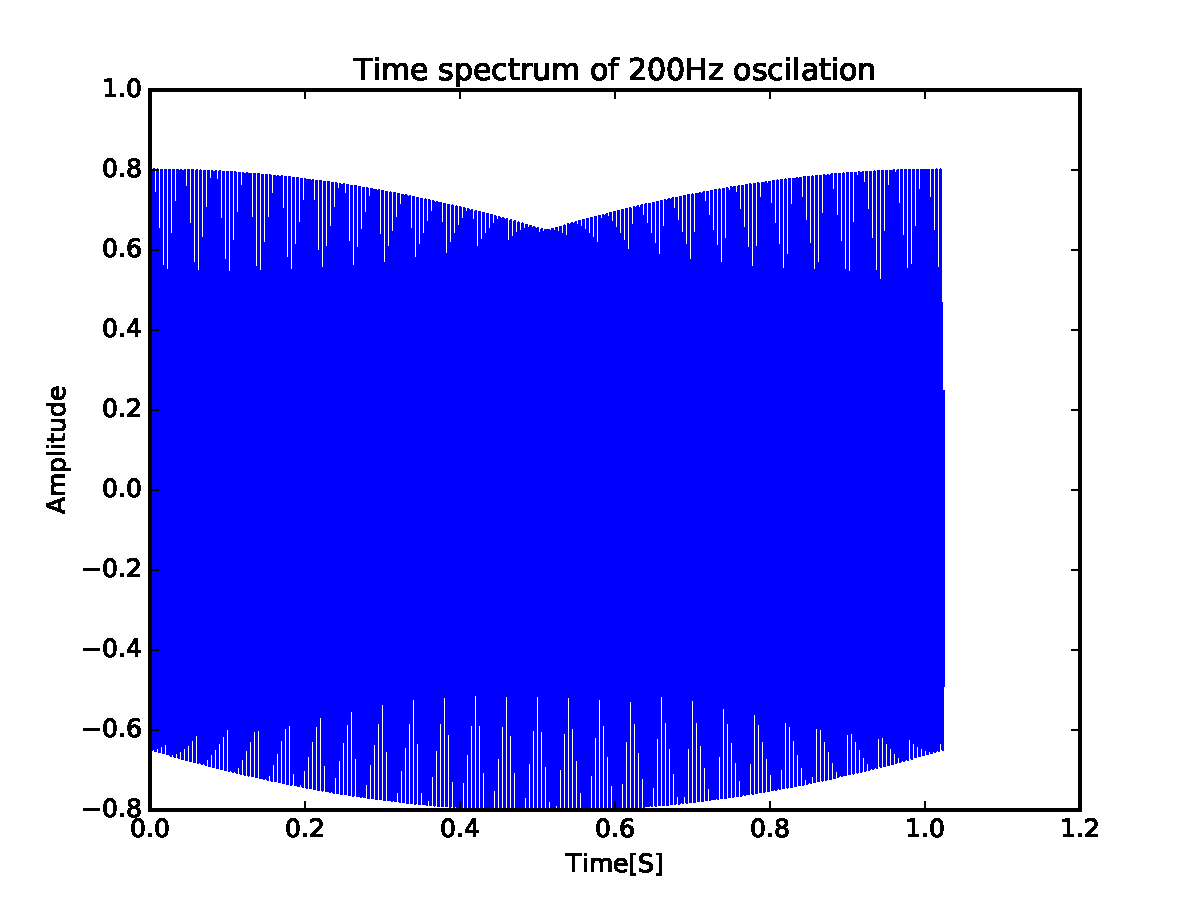
\includegraphics[width=0.49\textwidth]{fig/timespec200.pdf}
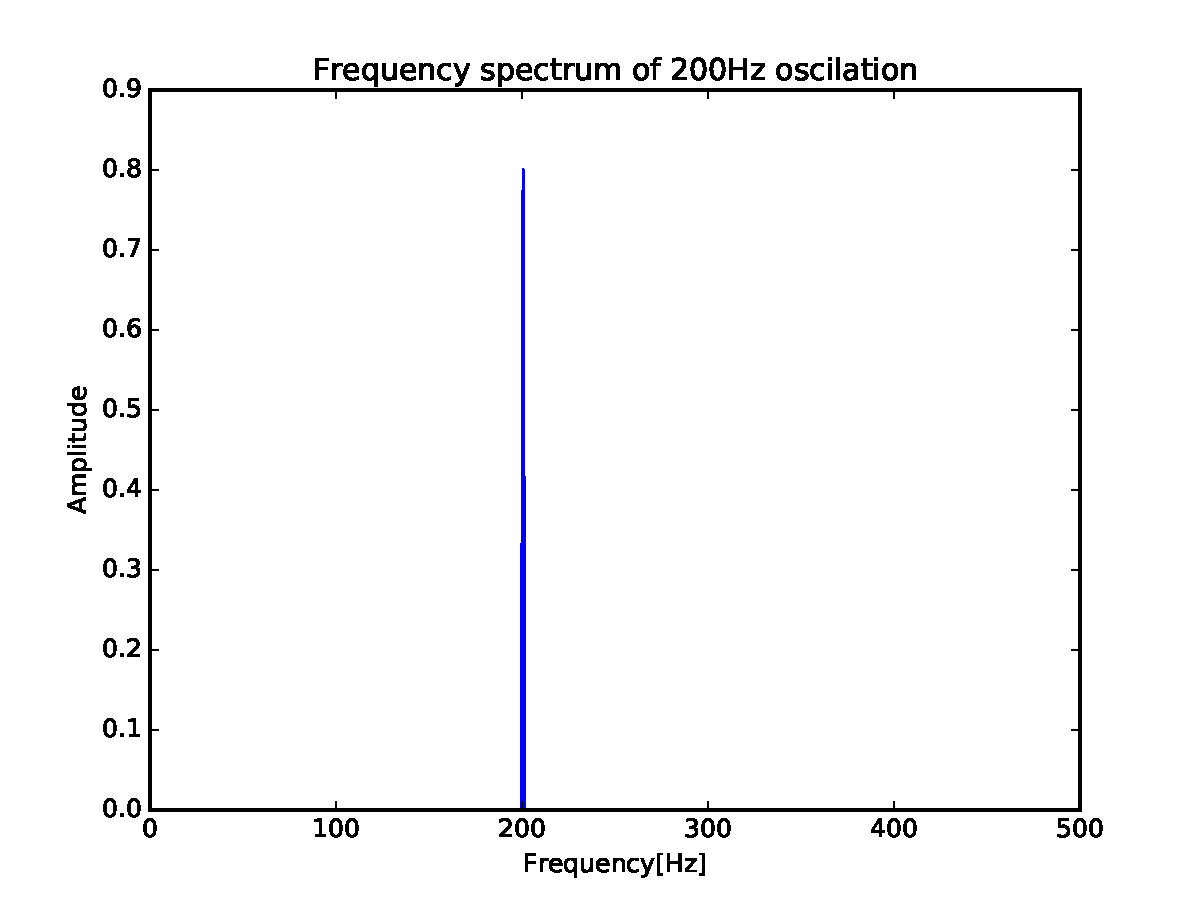
\includegraphics[width=0.49\textwidth]{fig/freqspec200.pdf}
\caption{Tids- og frekvensspekter av 200Hz svingning}
\end{figure}
\begin{figure}[H]
\centering
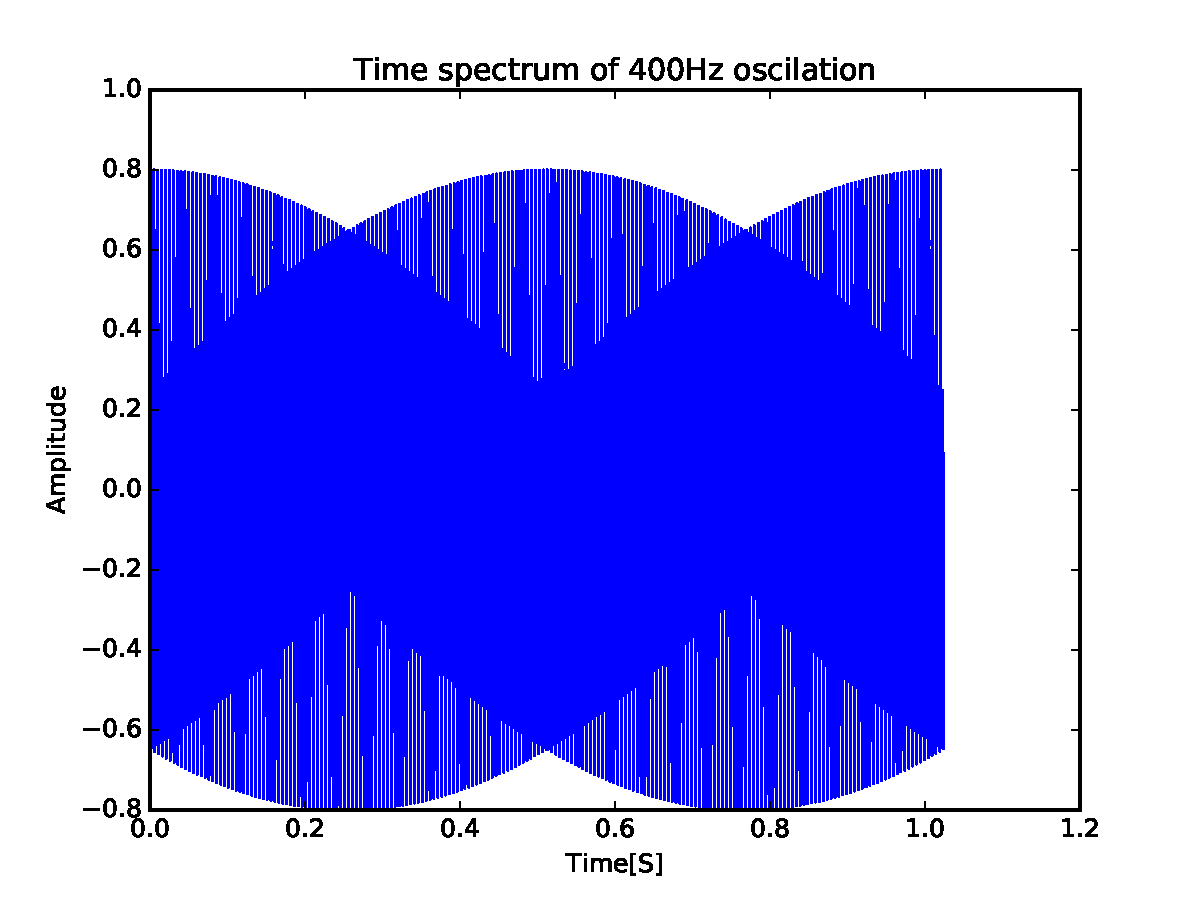
\includegraphics[width=0.49\textwidth]{fig/timespec400.pdf}
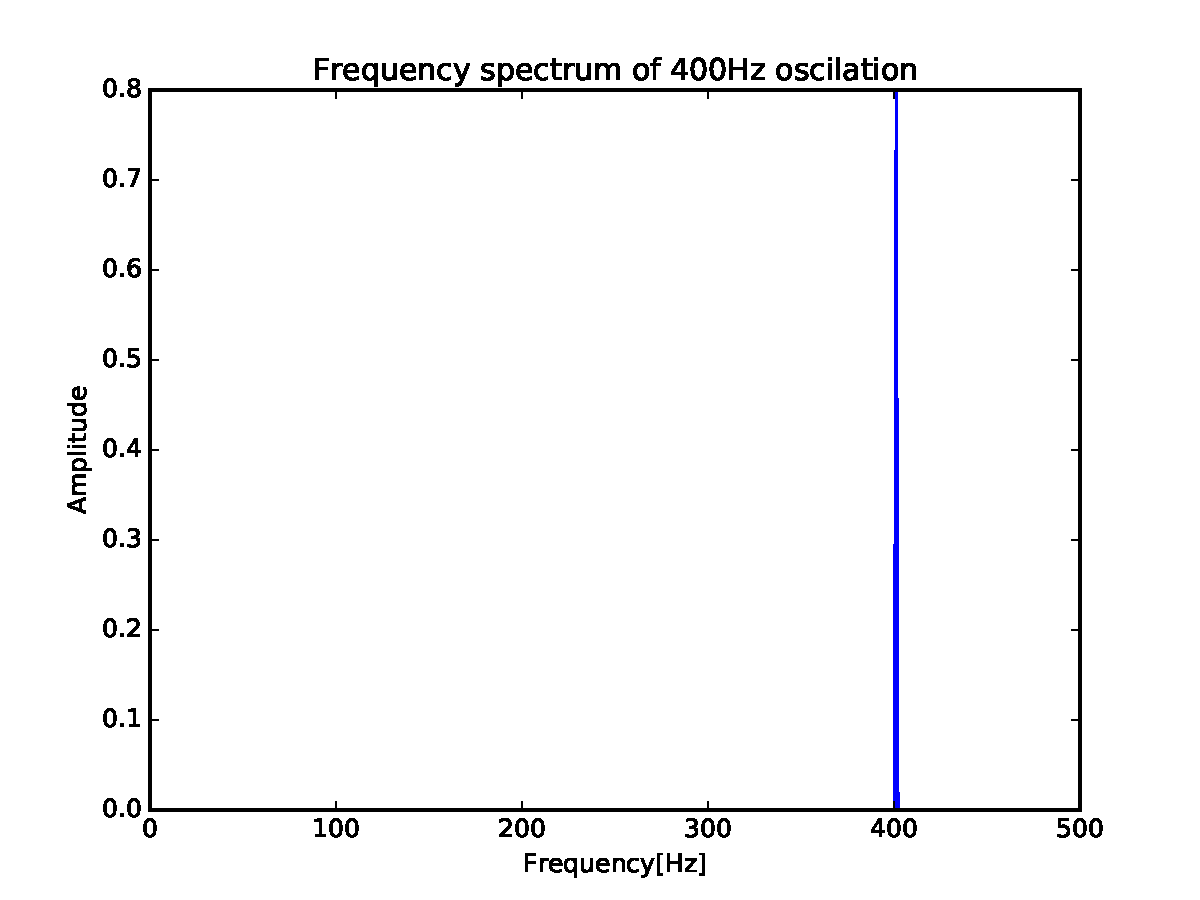
\includegraphics[width=0.49\textwidth]{fig/freqspec400.pdf}
\caption{Tids- og frekvensspekter av 400Hz svingning}
\label{fig:400Hz}
\end{figure}
\begin{figure}[H]
\centering
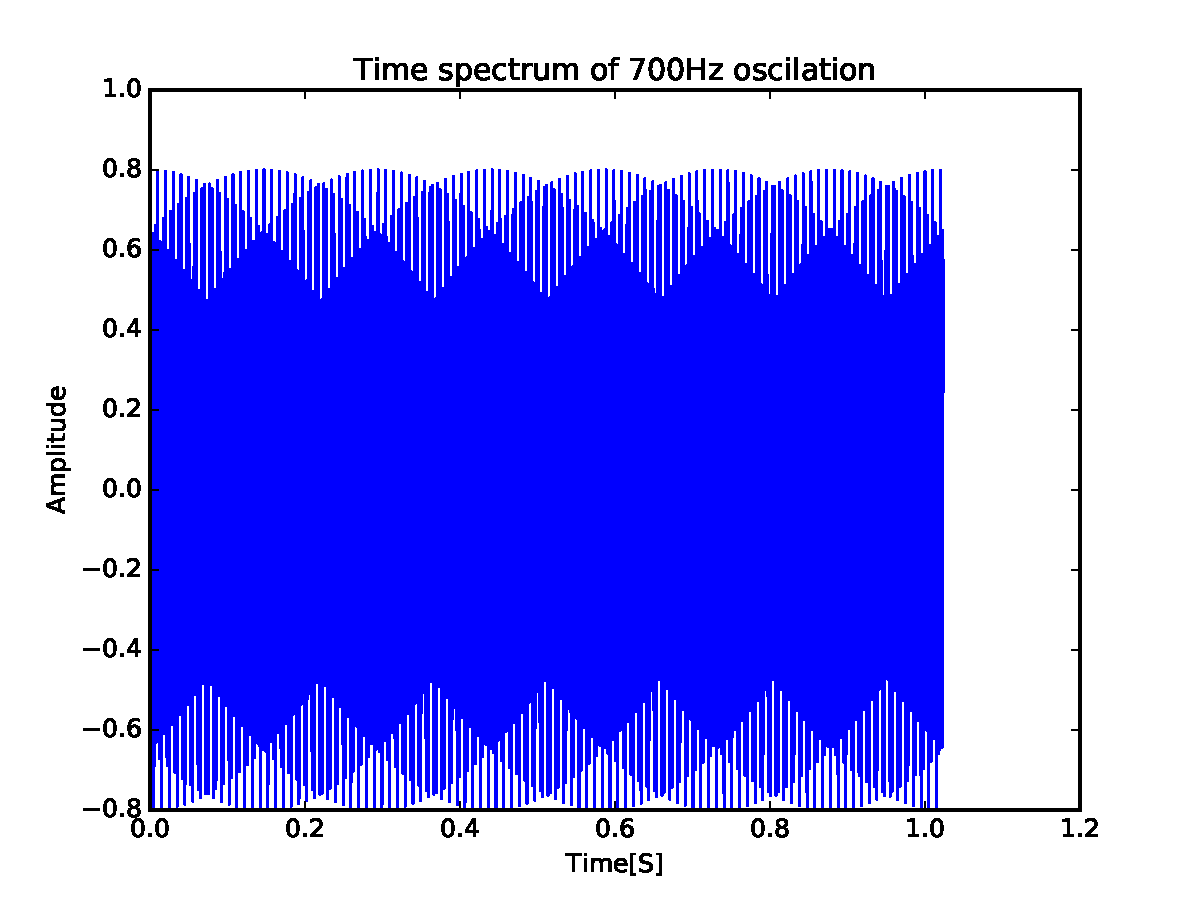
\includegraphics[width=0.49\textwidth]{fig/timespec700.pdf}
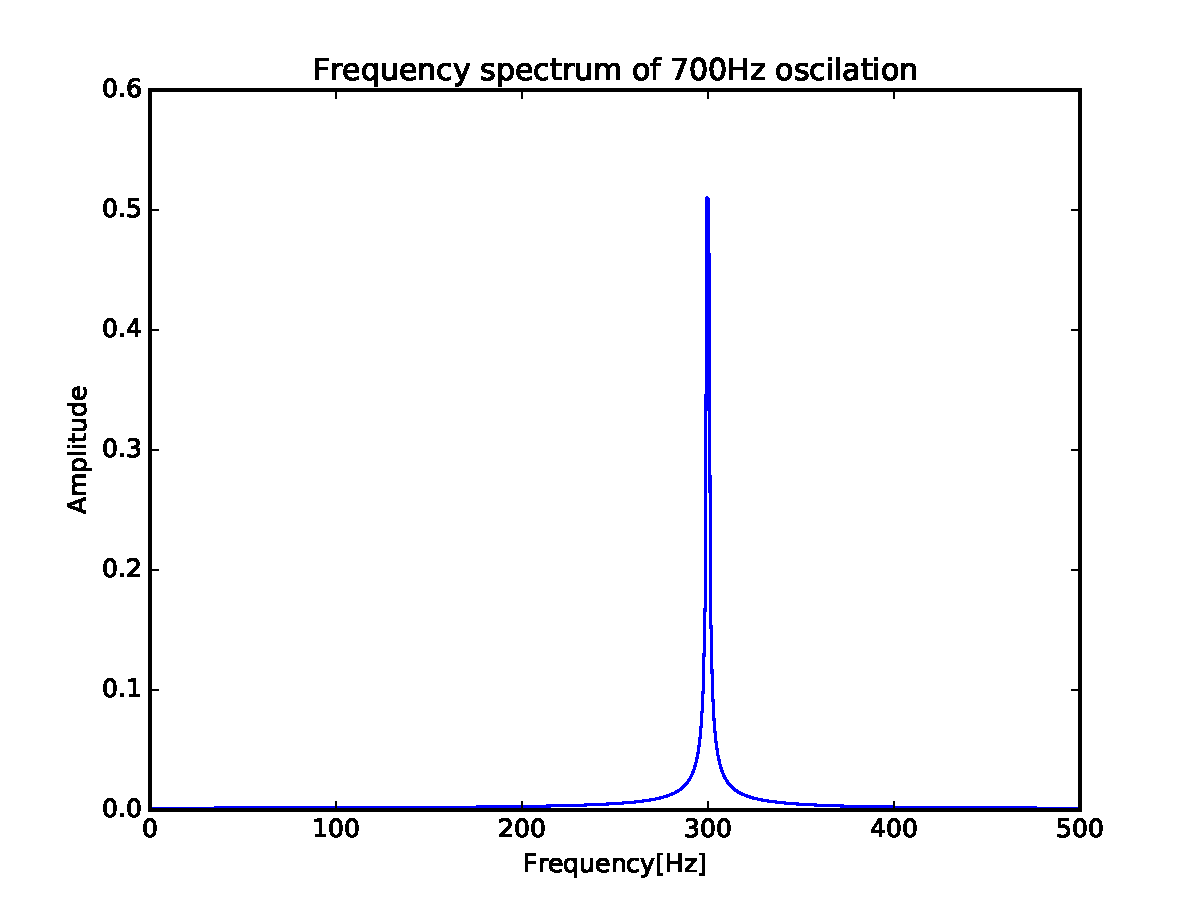
\includegraphics[width=0.49\textwidth]{fig/freqspec700.pdf}
\caption{Tids- og frekvensspekter av 700Hz svingning}
\label{fig:700Hz}
\end{figure}
\begin{figure}[H]
\centering
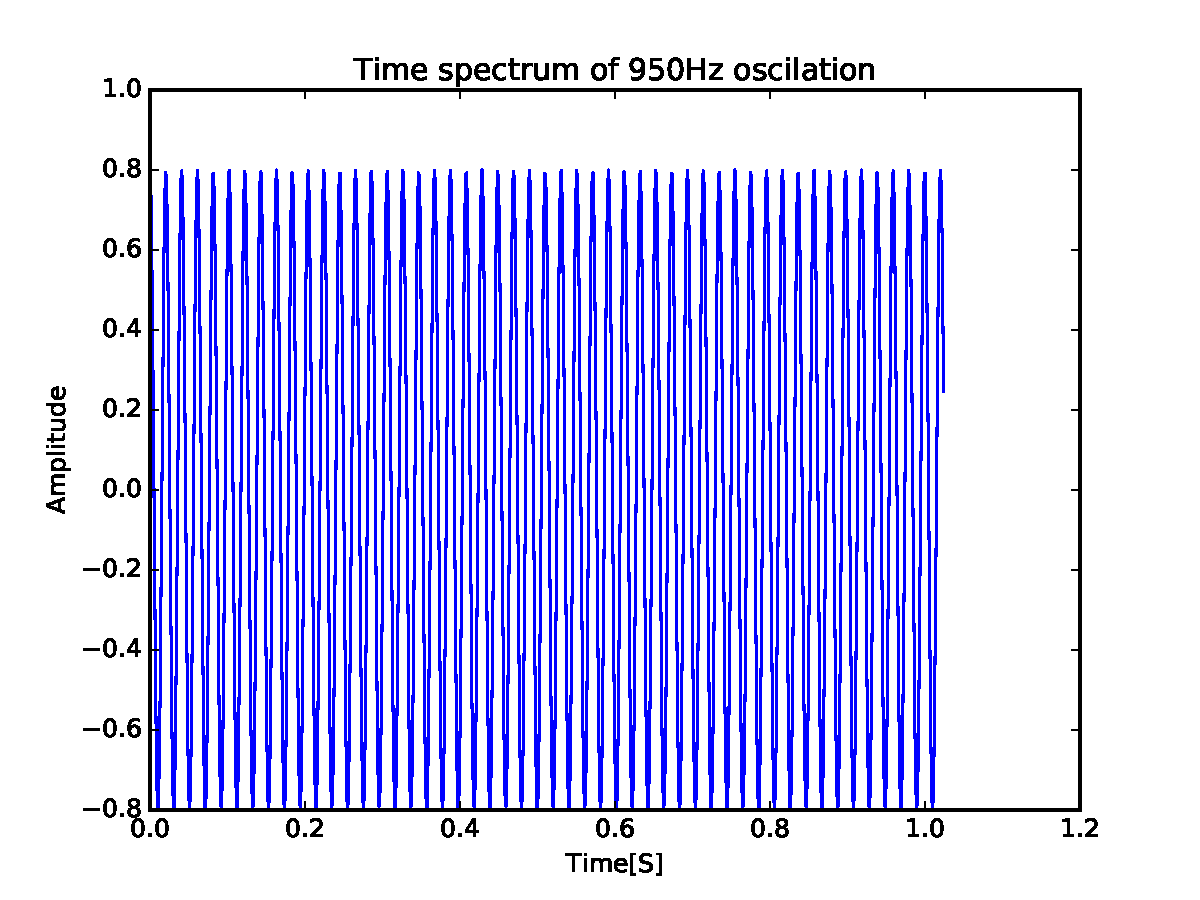
\includegraphics[width=0.49\textwidth]{fig/timespec950.pdf}
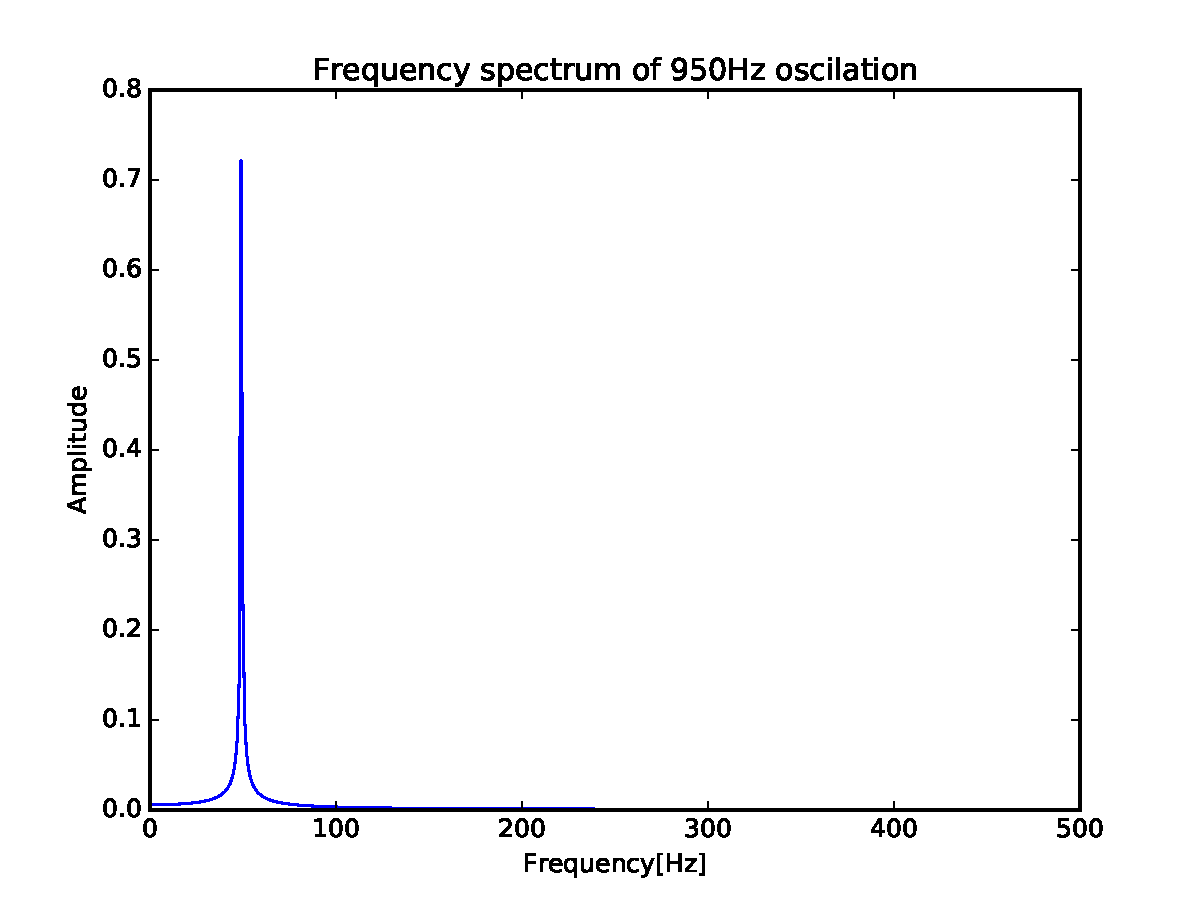
\includegraphics[width=0.49\textwidth]{fig/freqspec950.pdf}
\caption{Tids- og frekvensspekter av 950Hz svingning}
\end{figure}
\begin{figure}[H]
\centering
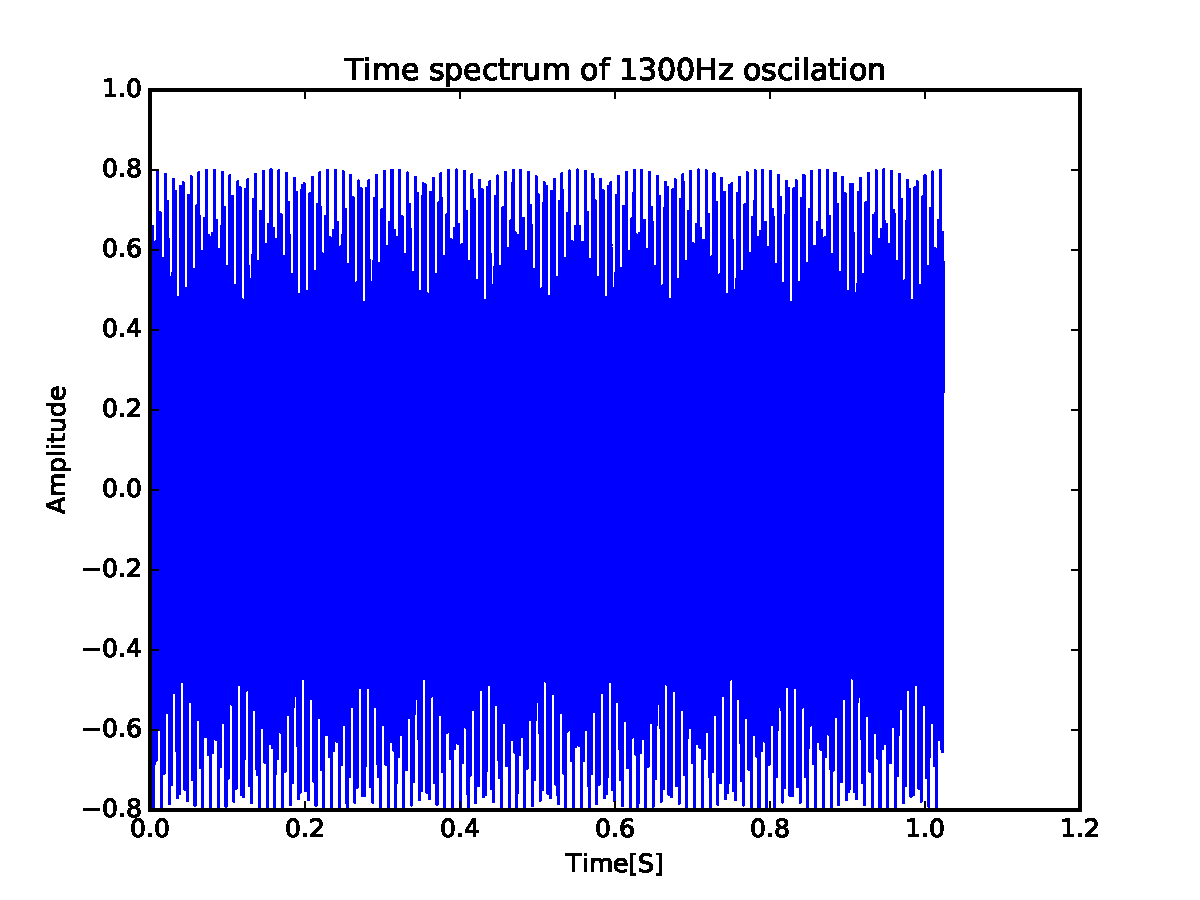
\includegraphics[width=0.49\textwidth]{fig/timespec1300.pdf}
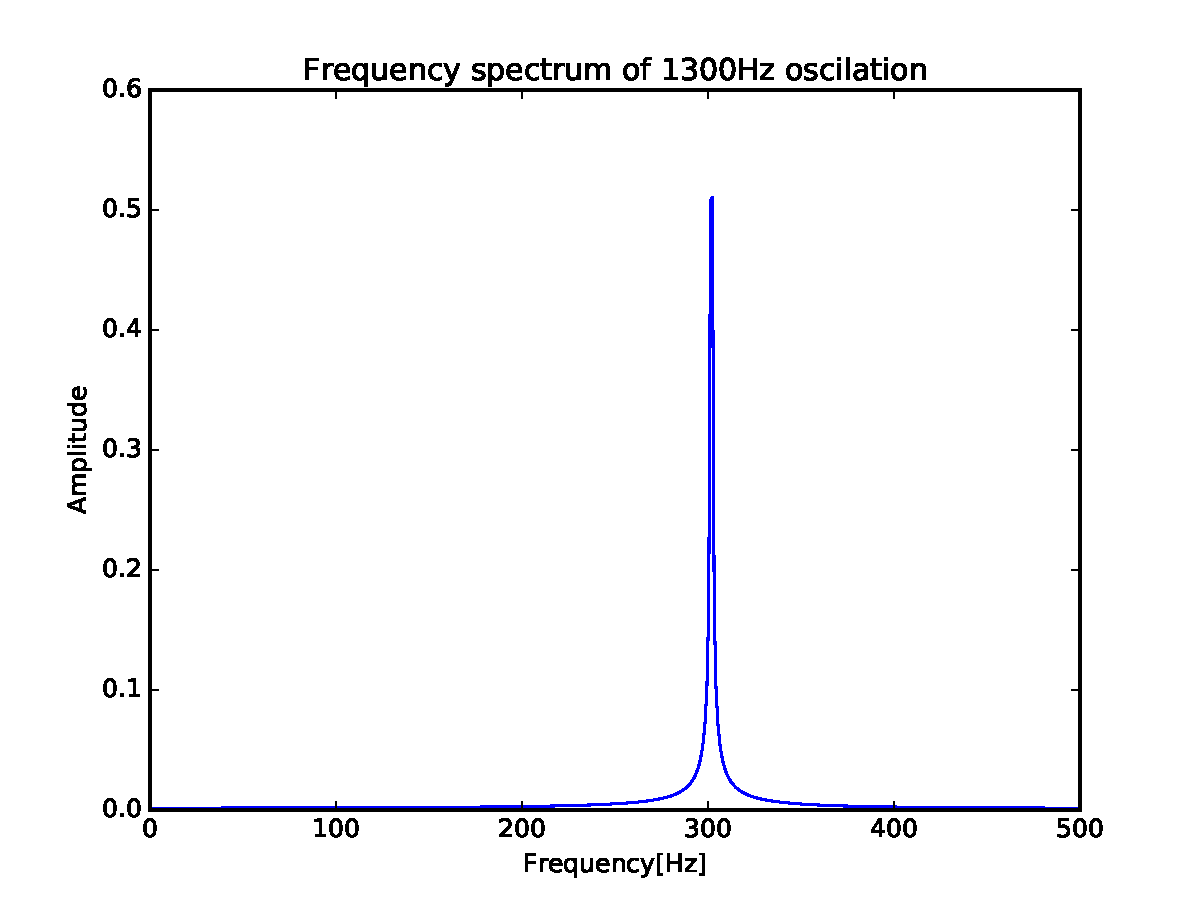
\includegraphics[width=0.49\textwidth]{fig/freqspec1300.pdf}
\caption{Tids- og frekvensspekter av 1300Hz svingning}
\label{fig:1300Hz}
\end{figure}



\section*{Oppgave 11}

Vi ser at frekvensspekteret i figur \ref{fig:sunspots} ligner det i boken. Vi ser også at den har en topp rundt frekvensen 0.1, som tilsvarer en periode på 10år. Dette stemmer godt overens med tidsspekteret, der vi kan se at toppene kommer gjevnlig, og er rundt 10 hvert hundrede år.

\begin{figure}[H]
\centering
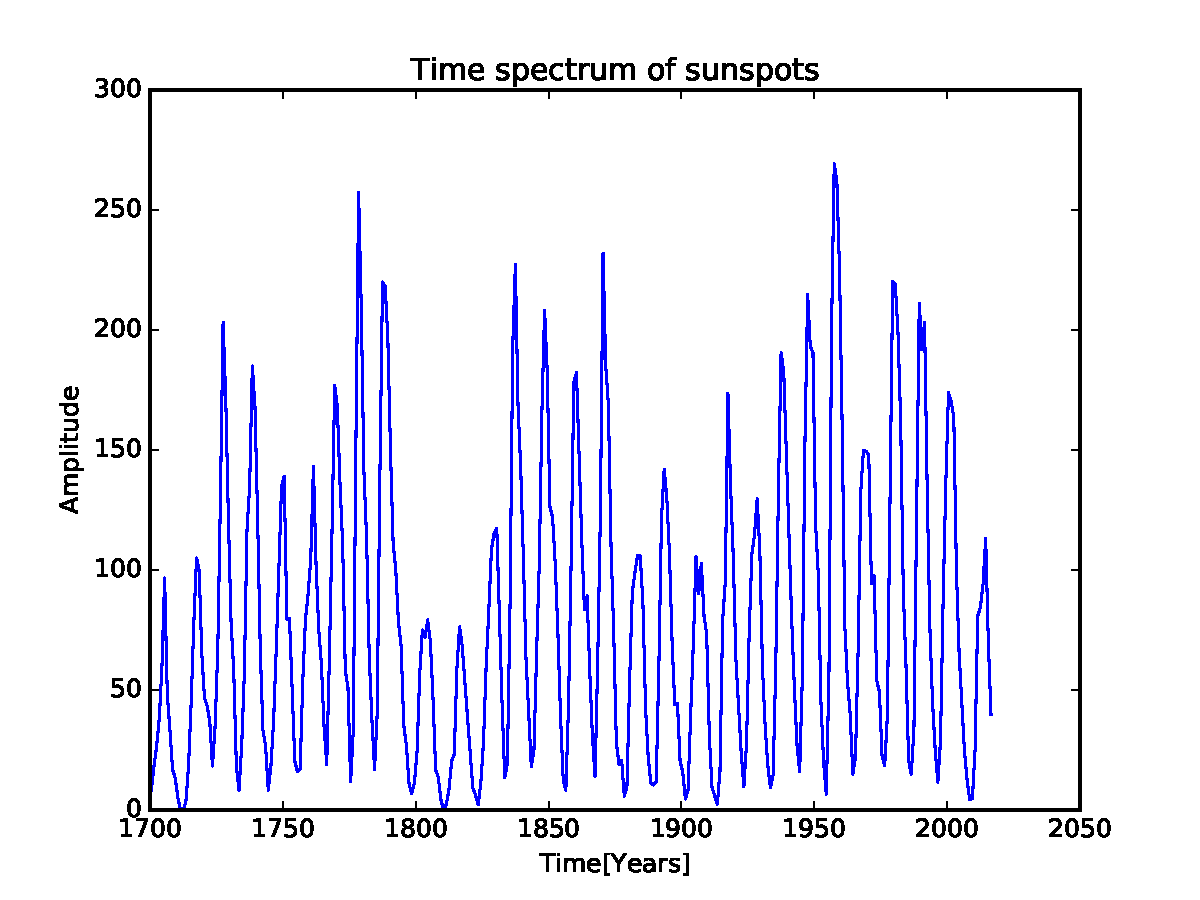
\includegraphics[width=0.49\textwidth]{fig/suntimespec.pdf}
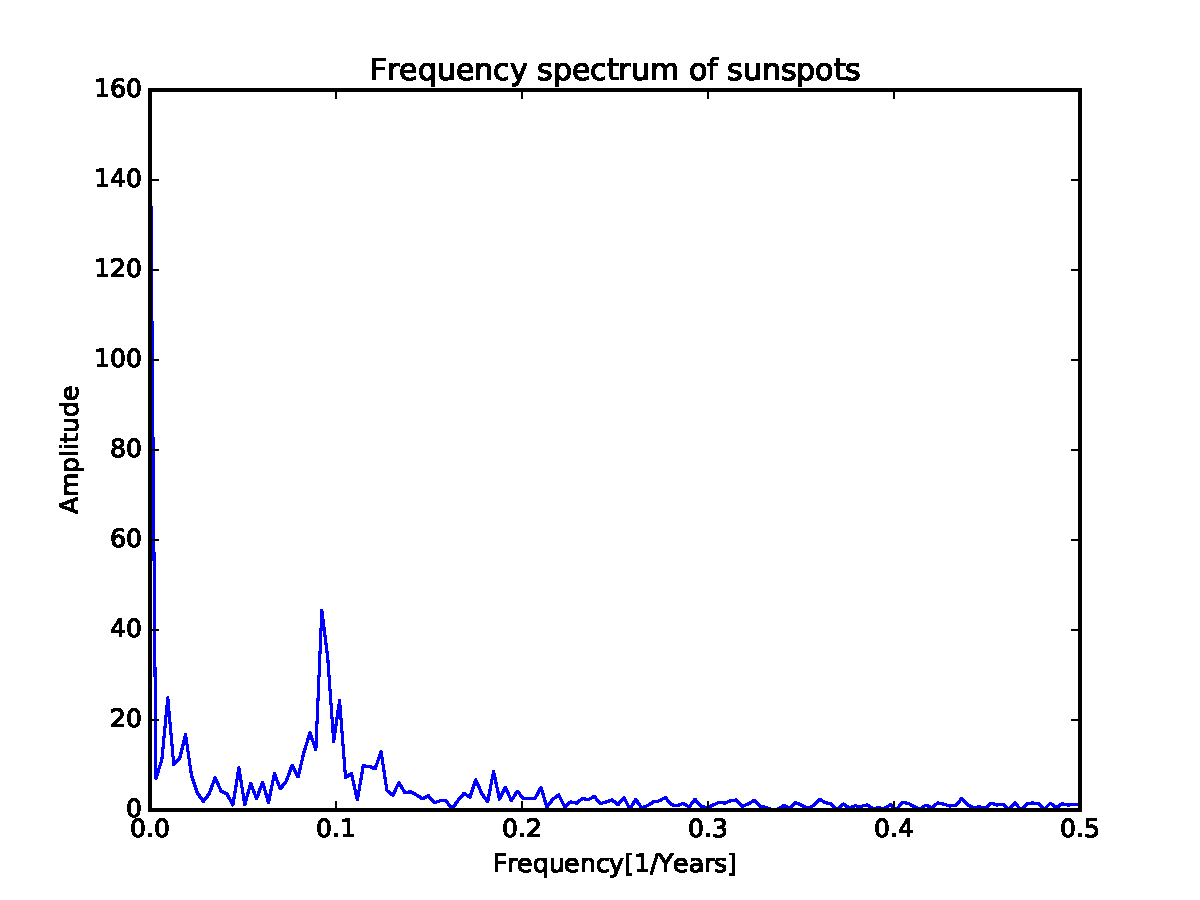
\includegraphics[width=0.49\textwidth]{fig/sunfreqspec.pdf}
\caption{Tids- og frekvensspekter til solflekk-data.}
\label{fig:sunspots}
\end{figure}




\section*{Oppgave 14 og 15}

Fra frekvensspekteret i figur \ref{fig:13} ser vi at 13 perioders signalet får en skarpere topp, som tilsvarer en tydeligere definert frekvens, enn 13.2 perioders signalet. Dette er fordi heltallet perioder gjør den til en fullstendig periodisk funksjon, også i ytterpunktene, mens den andre funksjonen vil ha litt udefinert periode helt i starten og slutten av plottet.

\begin{figure}[H]
\centering
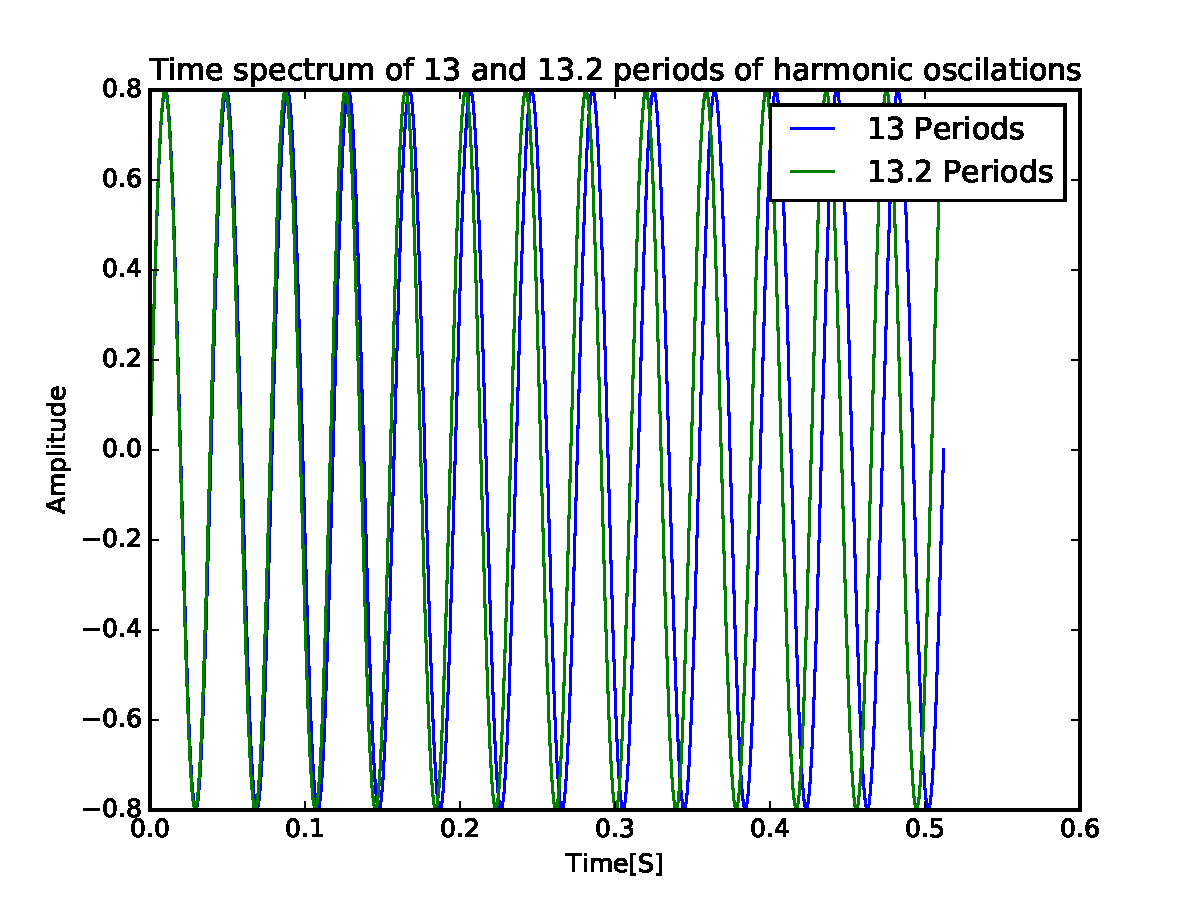
\includegraphics[width=0.49\textwidth]{fig/timespec.pdf}
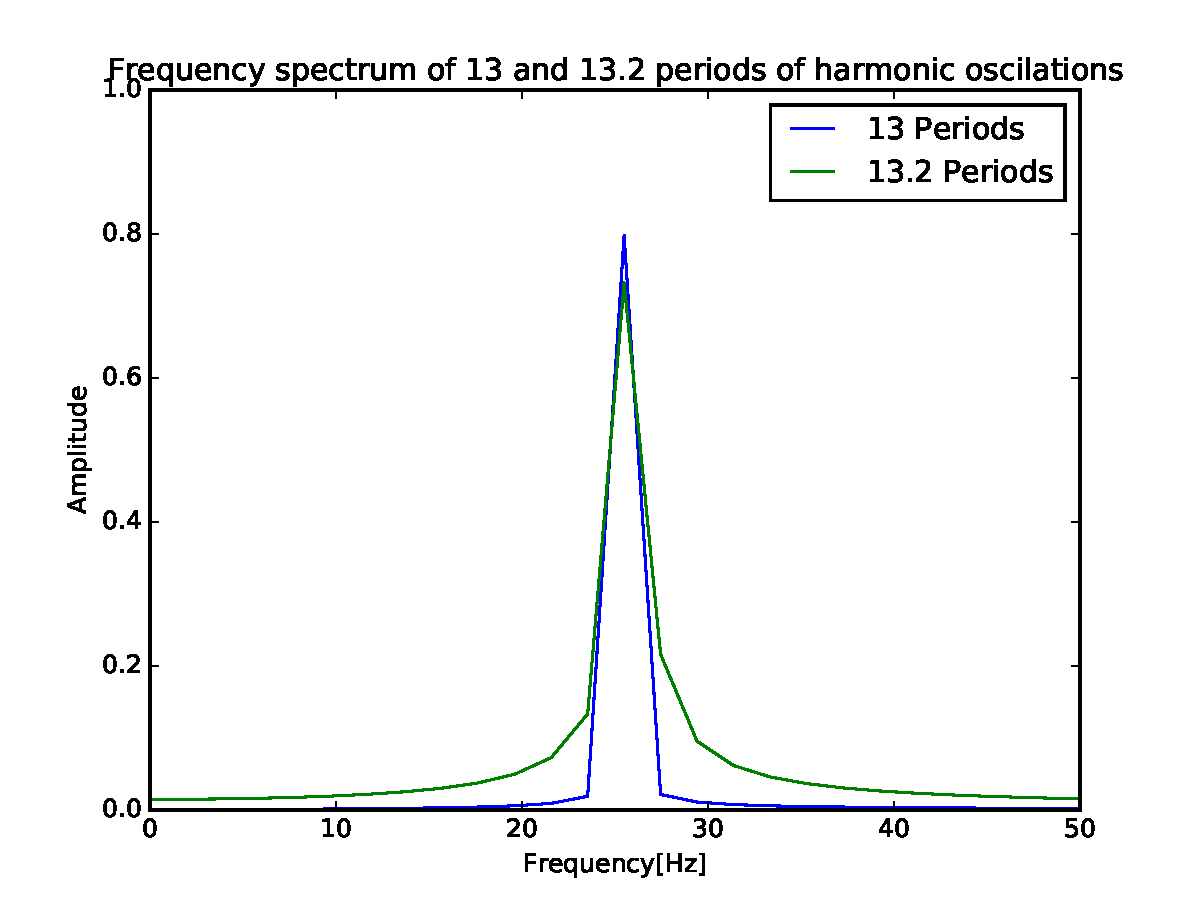
\includegraphics[width=0.49\textwidth]{fig/freqspec.pdf}
\caption{Tids- og frekvensspekter til 13 og 13.2 perioders sinus-svingninger.}
\label{fig:13}
\end{figure}



\section*{Oppgave 16}

Vi ser fra figur \ref{fig:square_timespec} at vi får firkant-mønsteret vi ønsker, med 16 perioder. Det fullstendige frekvensspekteret i figur \ref{fig:square_freqspec1} kan være litt vanskelig å tolke, så jeg har inkludert en zoom'et versjon i figur \ref{fig:square_freqspec1}. Her ser vi at vi har tydelig definerte oddetalls-frekvenser, 1, 3, 5, 7,..., som avtar i amplitude.

En slik pulsrekke vi ser i tidsbildet kan modelleres som en uendelige rekke av harmoniske svingninger, på formen
\begin{align*}
x(t) = \sin{t} + \frac{1}{3}\sin(3t) + \frac{1}{5}\sin(5t) + \frac{1}{7}\sin(7t) + \cdots
\end{align*}
(her kan det inkluderes en rekke konstanter, men den fundamentale formen koker ned til dette).

Vi ser at dette stemmer overens med både de frekvensene vi ser, og den avtagende amplituden på frekvensene.

\begin{figure}[H]
\centering
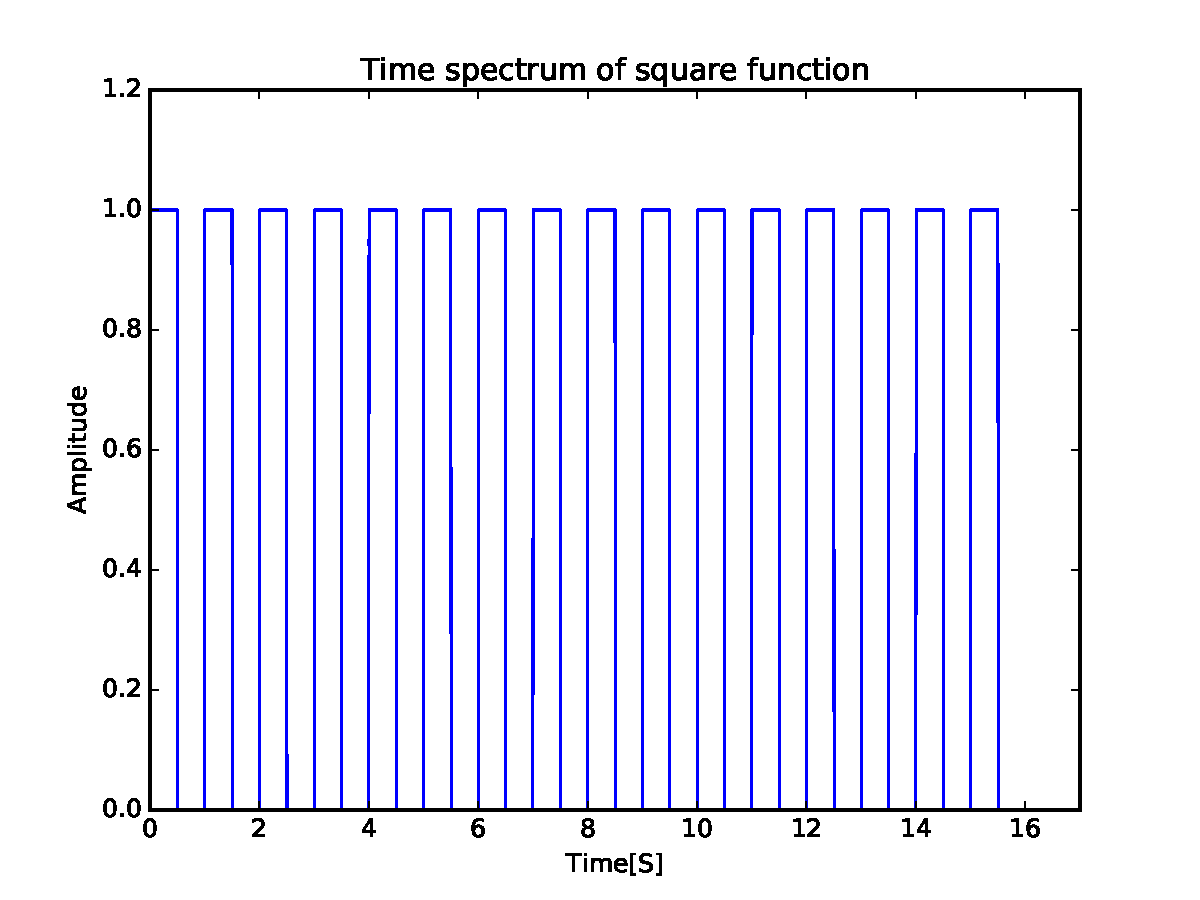
\includegraphics[width=0.8\textwidth]{fig/squaretimespec.pdf}
\caption{Tidsspekter til firkant-funksjon}
\label{fig:square_timespec}
\end{figure}

\begin{figure}[H]
\centering
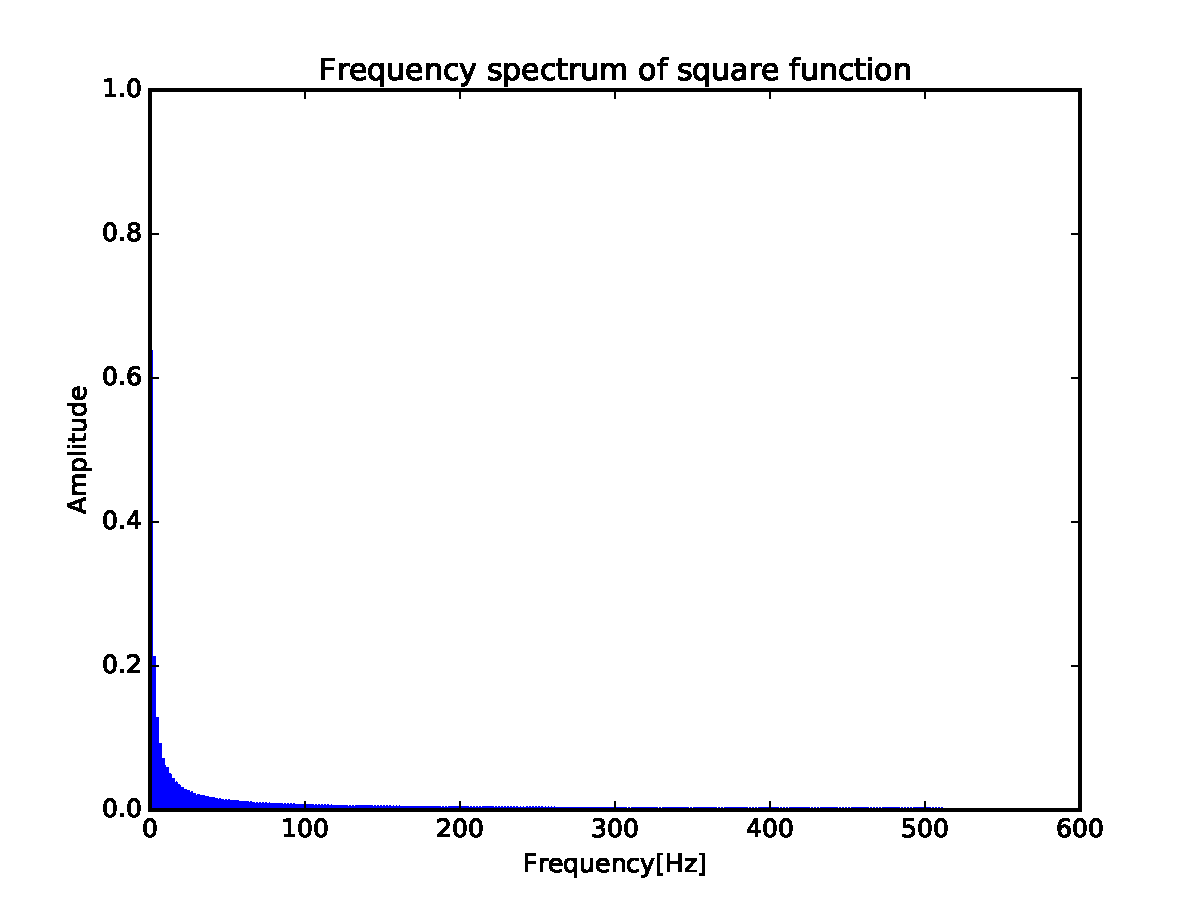
\includegraphics[width=0.8\textwidth]{fig/squarefreqspec1.pdf}
\caption{Frekvensspekter til firkant-funksjon}
\label{fig:square_freqspec1}
\end{figure}

\begin{figure}[H]
\centering
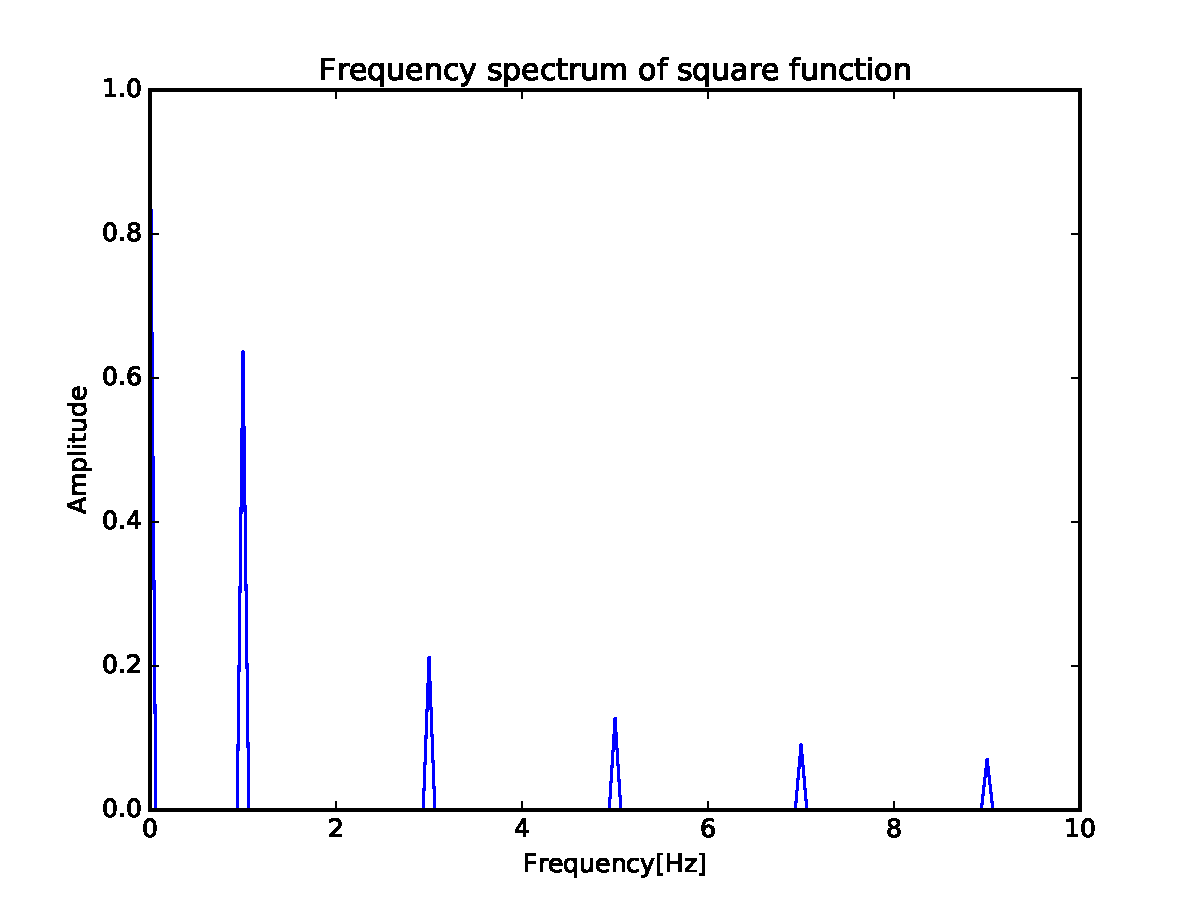
\includegraphics[width=0.8\textwidth]{fig/squarefreqspec2.pdf}
\caption{Frekvensspekter til firkant-funksjon, kuttet ved 10Hz}
\label{fig:square_freqspec2}
\end{figure}

















\end{document}
